\documentclass[10pt,a4paper]{article}
\usepackage[spanish]{babel}
%\usepackage[latin1]{inputenc}
%\usepackage[latin2]{inputenc}
\usepackage[utf8]{inputenc}
\usepackage[T1]{fontenc}
\usepackage{graphicx}
\usepackage{titling}
\date{\today}
\usepackage{fancyhdr}
%\pagestyle{fancy}
\fancyhf{}
%\lhead[\leftmark]{Nombre Autor}
%\rhead[Nombre Autor]{\rightmark}
%\lfoot[\thepage]{}
%\rfoot[\leftmark]{\thepage}
%\lfoot{\hline}
\usepackage{tikz}
\usetikzlibrary{shapes.geometric, arrows}

\tikzstyle{rec} = [rectangle, rounded corners, text centered, draw=black]
\tikzstyle{arrow} =[thick,->,>=stealth]
\tikzstyle{line} = [draw, -latex']

\begin{document}
\begin{titlepage}
	\centering
\begin{figure}[h]
\centering

\includegraphics[scale=0.2]{escudo.png}
\end{figure}
{\bfseries\LARGE Universidad Concepción \par}
\vspace{0.2cm}
{\scshape\Large Facultad de Ciencias Físicas y Matematicas\par}
\vspace{0.2cm}
{\scshape\Large Departamento de Física\par}
\vspace{3cm}
{\scshape \small{Informe 01:}\\ \Huge Modelo basado en agentes\\Modelo LLS  \par}
\vspace{3cm}
{\itshape\Large Informe de Tesis II (510602)\par}
\vfill
{\Large Autor: \par}
{\Large Mauricio Lagos Morales \par}
\vfill
{\Large \thedate \par}		
\end{titlepage}
\section*{Introducción}\label{Introduccion}
	\subsection*{Presentación tema y obejticos del informe}
\quad En este informe se presenta el primer avance del curso actual (Tesis II). Se utilizará el modelo basado en agentes propuesto por Levy, Levy y Solomon \cite{Levy1994} para describir el mercado financiero, en el modelo se que describen un conjunto (ensemble) de agentes financieros interactuando con un simple obejtivo de maximizar su utilidad esperada en una simple dinámica de oferta y demananda .\\ 
\quad El principal objetivo de este informe, es presentar el modelo del cual se pretende realizar un trabajo más exhaustivo y complejo. Y se entrega los primeros resultados obtenidos en la implemantación del modelo base en Python 3, y la similitud  y diferencias con los datos obtenidos en la primera referencia literaria \cite{Levy1994}.
\subsection*{Describir el caso}
\quad El modelo presetado en \cite{Levy1994} consiste en un conjunto de $i$ de agentes financieros, interactuando de una mercado financiero, con el objetivo de maximizar su utilidad esperada.\\
\quad En cada paso de tiempo $t$, cada inversor, $i$  debe dividir su riqueza $w_i(t)$ entre activos con riego (acciones) y activos seguros (bonos). Mediante un factor de inversion $x(i)$ el cual podrá variar, permitiendo que el modelo cambie; desde un modelo donde todos los individuos eligen de la misma forma (versión homogenea) a diferenciarse entre ellos en la la forma de elegir cuantas acciones podran comprar ( versión heterogenea), haciendo que el modelo sea mucho mas realista.
\subsection*{Explicar el problema estudiado}
\quad Se presentará los resultados del modelo base que se logro implementar. El modelo parte siendo homogeneo y continua hacia la heterogeneidad aumentando levemente el valor de la aletoridad.
\subsection*{Explicar la metodologia}
\quad Se implementará el modelo basado de agentes en Pycharm, que usa librerias Python 3.8, El modelo implementado se puede resumir en Tab. [\ref{Diagrama}], las condiciones básicas son sacadas directametne de \cite{Levy1994}


\begin{figure}[ht]
	\centering
	\begin{tikzpicture}[node distance = 1.3cm,auto]
		\node (eleccion) [rec] {Elección de};
		\node (opt) [rec, below of=eleccion] {Optimización};
		\node (ruido) [rec, below of=opt] {Agregar ruido a la elección};
		\node (cod) [rec, below of=ruido] {Calcular el Precio};
		\node (historial) [rec, below of= cod] {Actualizacion del Historial};
		\node (actualizar) [rec, below of= historial] {Distribución de intereses y dividendos};
		\node (fin) [rec, below of= actualizar] {Termino tiempo t};
		\draw [line] (eleccion) -- (opt);
		\draw [arrow] (opt) -- (ruido);
		\draw [arrow] (ruido) -- (cod);
		\draw [arrow] (cod) -- (historial);
		\draw [arrow] (historial) -- (actualizar);
		\draw [arrow] (actualizar) -- (fin);
%		\draw [line] (fin) |- (eleccion);
%		\path [line] (fin) -| (eleccion);
	\end{tikzpicture}	
	\caption{Diagrama de flujo de la dinámica del programa}
	\label{Diagrama}
\end{figure}

\section*{Marco Teorico}\label{Marco Teorico}
	\subsection*{Física y Economía}

\subsection*{Racionalidad limitada}


\subsection*{Modelo Levy-Levy-Solomon}\label{mlls}
\quad El modelo propuesto por Levy, Levy y Solomon \cite{Levy1994} en 1994 consiste en un
 ensemble de agentes financieros $i$ que intereactuan en un mercado financiero y tienen dos opciones de invertir su riqueza total $w(i)$; un activo sin riesgo (\textbf{bonos}) y una activo con riesgo (\textbf{acción}).\\
\quad Al final de cada periodo de transacción el rendimiento de los bonos se retribuido von un retorno $r$ constante que se actualiza cada año. Además, las acciones tienen un dividendo denotado por $D$.\\
\quad Para poder elegir la opcion de inversión $x(i)$, cada agente recurre a los últimos $k$ retornos del mercado $H(j)$que recuerda para elegir la mejor ocpión para poder maximizar su riqueza. Los inversores creen que cada uno de estos $H(j)$ tiene una propabilidad de reaparecer de $1/k$.\\
\quad Entonces, en un comienzo cada todos los inversores cuentan con la misma riqueza $w$.\dots\\
\quad Al comienzo de $t$, el agente elige un precio hipotetico $P_h$ del historial de los retornos, con esto es posible calcular una riqueza hipotetica
\begin{equation}
	w_h(i)= w_0(i)+N_0(i) (P_h-P_0)\label{wh}
\end{equation}
donde $N_0(i)$ son las acciones que el agente $i$ le son entregadas al inicio de la simulación. Con $P_h$ y $w_h$ es posible calcular la cantidad de acciones a invertir $x(i)$ maximizando la utilidad esperada,
\begin{equation}
	EU[x(i)]=\frac{1}{k}\sum^{k}_{j=1}\log[(1-x(i))w_h(i)(1+r) + x(i)w_h(i)(1+H(j))]\label{mue}
\end{equation}
al obtener el valor $x(i)$, que es igual para todos en el mercado, se le agrega un factor de ruido que hace que cada elecion difiera entre cada uno de los agentes
\begin{equation}
	\tilde{x}(i)= x(i)+\varepsilon(i) \label{ruido}
\end{equation}
Ahora se calcula, la cantidad de acciones que cada uno de los inversores podrá mantener,
\begin{equation}
	N_h(i)=\frac{x(i)w_h(i)}{P_h}\label{nh}
\end{equation} 
esto creará la curva de demanda personal de cada agentes. Ahora, para obtener el precio en el actual paso temporal $t$, se utiliza la condicion de mercado ("\textit{clearence market}"). Al sumar todas las curvas de demandas, numero de acciones, se obtiene las acciones totales del mercado, pero este número es fijo $N_A$
\begin{equation}
	N_A=\sum^{N}_{i=1}N_h(i)\label{ccm}
\end{equation}
y el precio se calcula
\begin{equation}
	P(t) = {\sum(\tilde{x}(i)w_h(i))}{N_A}
\end{equation}
Con esto la riqueza de cada inversor cambia
\begin{equation}
	w_1(i)= w_0(i)+N_0(P_1-P_0)
\end{equation}
y el número de acciones es
\begin{equation}
	N(i)=\frac{X_i(i)W(i)}{P(t)}\label{aciones}
\end{equation}
con esto ahora, pasamos al etapa de resdistribución de dividendos e intereses
\begin{equation}
	w_1(i) = w_1(i) + (1-\tilde{x}(i))w_1(i)(1+r) + \tilde{x}(i)w_1(1)(1+d)
\end{equation}
Por último el nuevo precio $P(t)$ genera un nuevo retorno 
\begin{equation}
	H_n = \frac{P_t-P_{t-1}+d}{P_{t-1}}
\end{equation} 
y este valor se ingresa al historial elimimando el mas antiguo de los valores. Con esto se termina una ronda de la simulación. 

\section*{Implementación}\label{Implementacion}
	Se implemente el modelo descrito más arriba, en Python 3.8. Los datos no ha sido refinado.\\
\quad Se utilizan los mismo datos que en \cite{Levy1994}, Periodo de tiempo un año ($256$ días habiles), con interés anual de $0,1$ (ó $10\%$). El Historial $0$, consiste de $k=10$ observaciones, con promedio $\mu=0.1001$ y con una $\sigma = 0.024$. En la ronda cero $x_0=50\%$.\\
\quad El número de inversores es asumido a ser $N=100$ y el numero de acciones total $N_A = 10.000$. La riqueza inicial de laca inversor es $w_0(i)=1.000$. El precio inicial dde las acciones es $P_0= 4.40$ y el dividendo $d= 0.3$. 

\section*{Resultados}\label{Resultados}
	\begin{figure}[h]
	\centering
	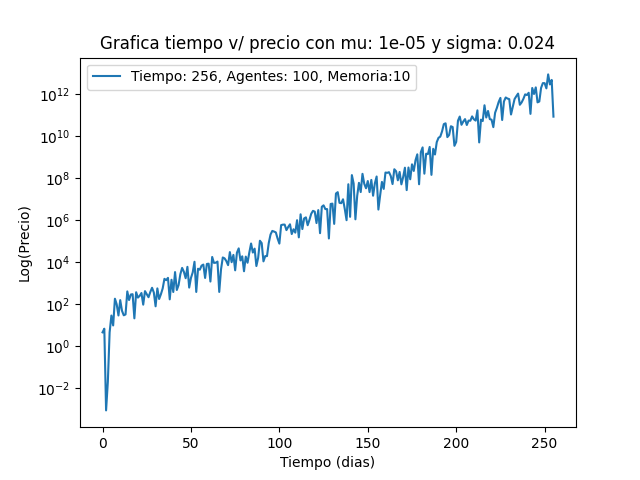
\includegraphics[scale=0.3]{fig_1a.png}\label{fig1}
	\qquad
	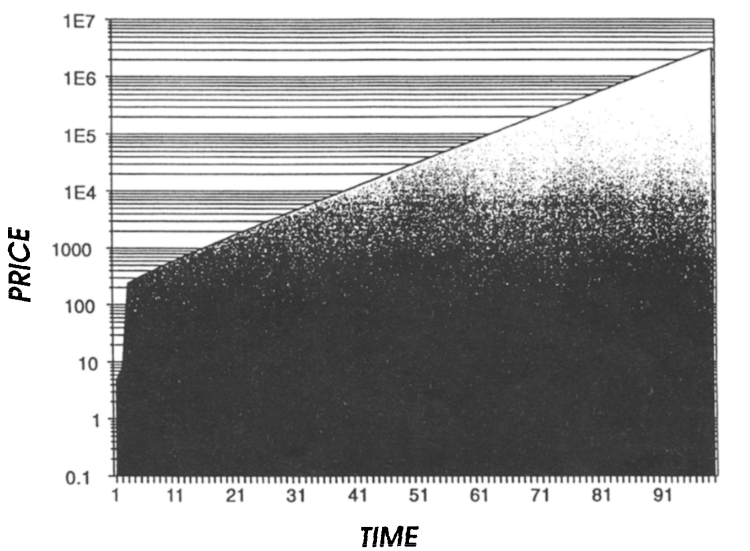
\includegraphics[scale=0.2]{fig_1b.png}\label{fig1b}
	\caption{$P(0) = 4.40$ y $\sigma = 0.00001$. \textit{Panel izquierdo} resultados optenidos en la simulacion, \textit{Panel derecho} resultados sacados del \cite{Levy1994}}
\end{figure}
\begin{figure}[h]
	\centering
	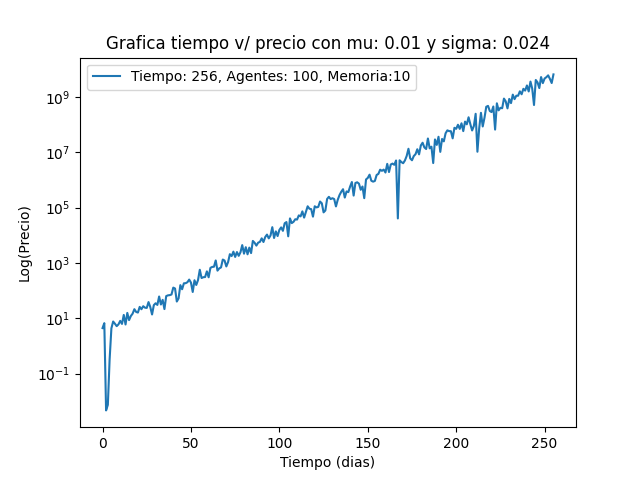
\includegraphics[scale=0.3]{fig_2.png}\label{fig2}
	\qquad
	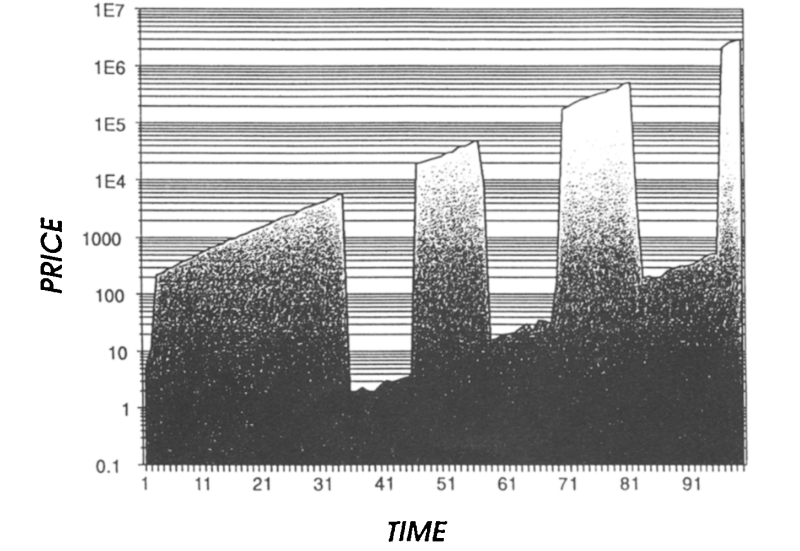
\includegraphics[scale=0.2]{fig_2b.png}\label{fig2b}
	\caption{$P(0) = 4.40$ y $\sigma = 0.01$. \textit{Panel izquierdo} resultados optenidos en la simulacion, \textit{Panel derecho} resultados sacados del 	\cite{Levy1994}}
\end{figure}
\begin{figure}[h]
	\centering
	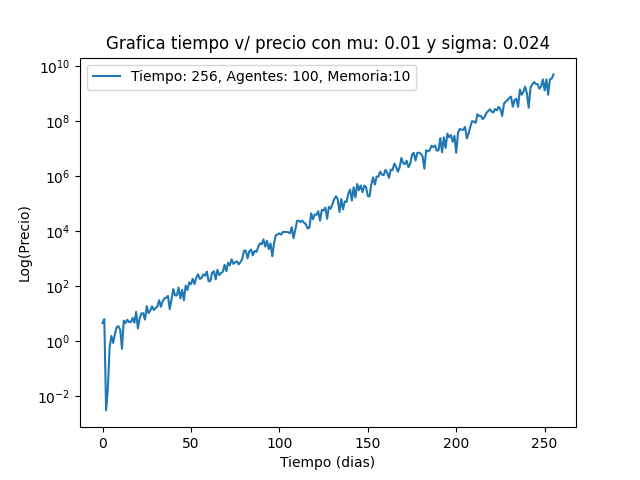
\includegraphics[scale=0.3]{fig_3.png}\label{fig3}
	\qquad
	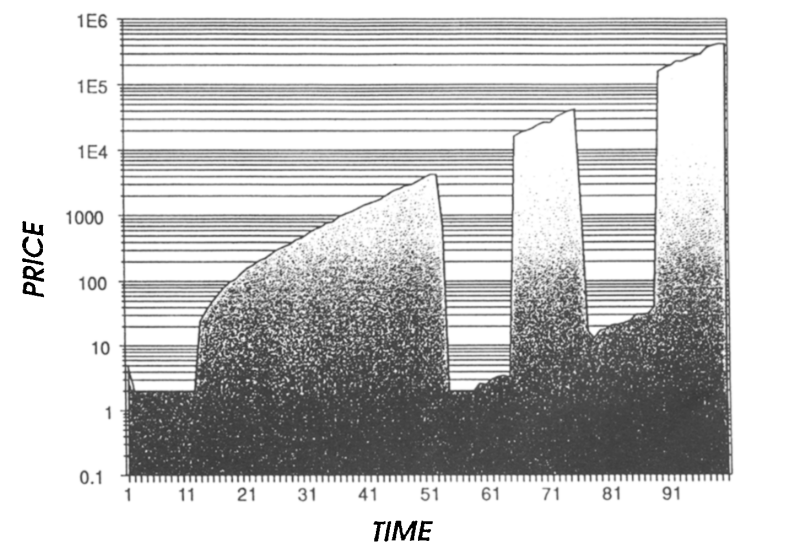
\includegraphics[scale=0.2]{fig_3b.png}\label{fig3b}
	\caption{$P(0) = 4.60$ y $\sigma = 0.01$. \textit{Panel izquierdo} resultados optenidos en la simulacion, \textit{Panel derecho} resultados sacados del \cite{Levy1994}}
\end{figure}
\begin{figure}[h]
	\centering
	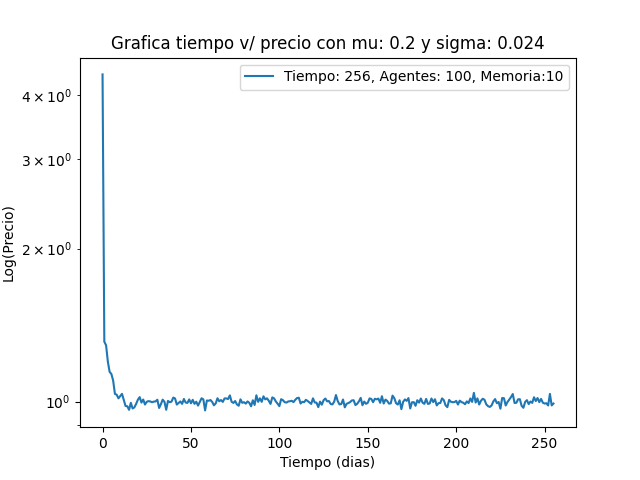
\includegraphics[scale=0.3]{fig_4.png}\label{fig4}
	\qquad
	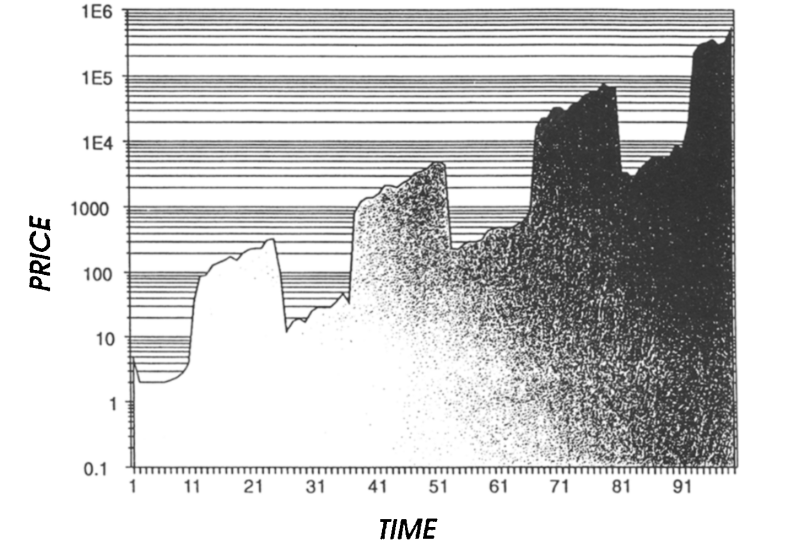
\includegraphics[scale=0.2]{fig_4b.png}\label{fig1b}
	\caption{$P(0) = 4.60$ y $\sigma = 0.2$. \textit{Panel izquierdo} resultados optenidos en la simulacion, \textit{Panel derecho} resultados sacados del \cite{Levy1994}}
\end{figure}
\begin{figure}[h]
	\centering
	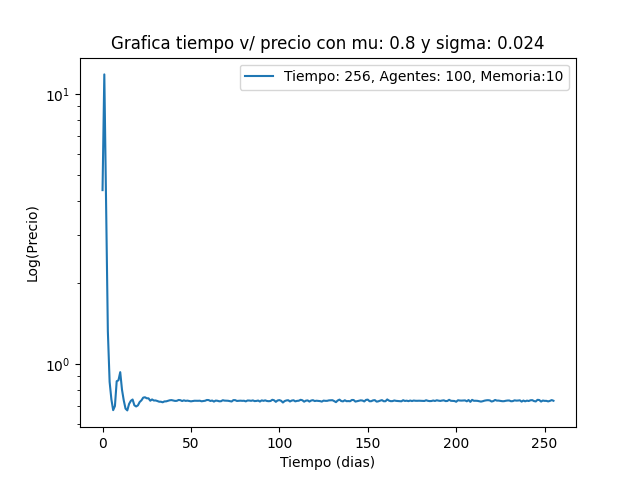
\includegraphics[scale=0.3]{fig_5.png}\label{fig5}
	\qquad
	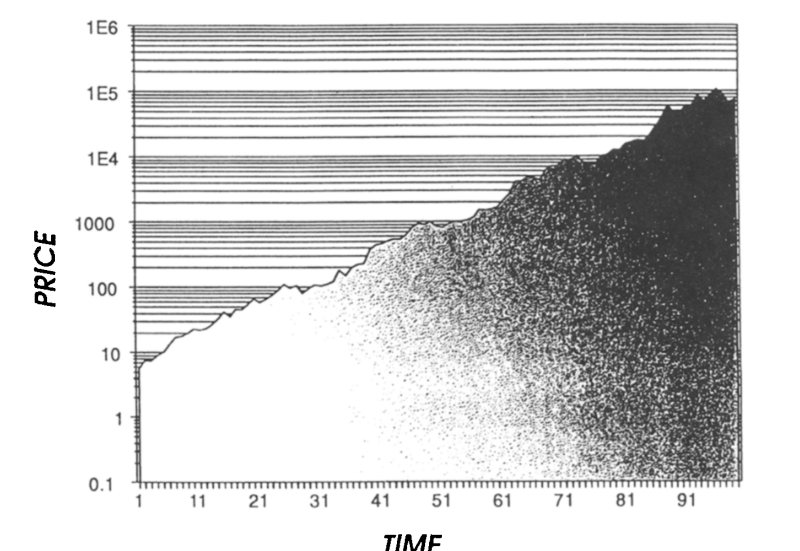
\includegraphics[scale=0.2]{fig_5b.png}\label{fig5b}
	\caption{$P(0) = 4.60$ y $\sigma = 0.8$. \textit{Panel izquierdo} resultados optenidos en la simulacion, \textit{Panel derecho} resultados sacados del \cite{Levy1994}}
\end{figure}
\section*{Conclusión}\label{Conclusión}
\bibliographystyle{unsrt} 
	\bibliography{biblio_00.bib}
\end{document}